\documentclass[10pt,a4paper]{article}
\usepackage[T1]{fontenc}
\usepackage[utf8]{inputenc}
\usepackage{lmodern}
\usepackage[a4paper,margin=16mm,headheight=15pt,footskip=18pt]{geometry}
\usepackage{microtype}
\usepackage{xcolor}
\usepackage{booktabs,tabularx,array,longtable}
\usepackage{siunitx}
\usepackage{fancyhdr,lastpage}
\usepackage{hyperref}
\usepackage{pgfplots}
\pgfplotsset{compat=1.18}
\definecolor{LabAccent}{HTML}{087F7B}
\definecolor{LabDark}{HTML}{0D2828}
\definecolor{LabSoft}{HTML}{F3F6F8}
\hypersetup{colorlinks=true,linkcolor=LabAccent,urlcolor=LabAccent,pdftitle={Mixed-Cation Validation Report},pdfauthor={Matteo Ginesi}}
\setlength{\parindent}{0pt}
\setlength{\parskip}{5pt}
\renewcommand{\arraystretch}{1.16}
\pagestyle{fancy}
\fancyhf{}
\fancyhead[L]{\textcolor{LabAccent}{\textbf{LABFLOW}}}
\fancyhead[R]{\small PRJ-2026-014-R01}
\fancyfoot[L]{\scriptsize University of Rome Tor Vergata · Pending researcher signature}
\fancyfoot[R]{\scriptsize Page \thepage\ of \pageref{LastPage}}
\renewcommand{\headrulewidth}{0.4pt}
\renewcommand{\footrulewidth}{0.4pt}
\newcommand{\metric}[3]{\begin{minipage}[t]{0.18\linewidth}\textcolor{LabAccent}{\scriptsize\bfseries #1}\\[-1pt]{\Large\bfseries #2}\\[-1pt]{\scriptsize #3}\end{minipage}}
\begin{document}
\begin{titlepage}
\color{LabDark}
{\small\bfseries\textcolor{LabAccent}{LABFLOW · SCIENTIFIC REPORT}}\par
\vspace{22mm}
{\Huge\bfseries Mixed-Cation Validation Report\par}
\vspace{3mm}
{\Large\color{LabAccent}Editable local report test\par}
\vspace{14mm}
\begin{tabularx}{\linewidth}{@{}>{\bfseries}lX@{}}
Project & PRJ-2026-014\\
Report code & PRJ-2026-014-R01\\
Author & Matteo Ginesi\\
Laboratory & CHOSE — Centre for Hybrid and Organic Solar Energy\\
Organisation & University of Rome Tor Vergata\\
Date & 2026-08-03\\
Approval & Pending researcher signature\\
Keywords & perovskite, mixed-cation, validation\\
\end{tabularx}
\vfill
\colorbox{LabSoft}{\parbox{0.95\linewidth}{\small This document is generated from the current LabFlow Report Composer state. Sections, author text, data selections and evidence follow the same canonical report model used by the live preview and native PDF.}}
\end{titlepage}

\section{Executive Summary}

The leading formulation remains FA0.90MA0.10.

\textbf{Research objectives.} Compare MA/FA ratios and identify the most stable high-efficiency device stack.

\begin{center}
\metric{BEST PCE}{21.28\%}{S08}
\hfill\metric{MEAN PCE}{19.79\%}{8 samples}
\hfill\metric{BEST STABILITY}{95\%}{retained}
\hfill\metric{MEAN VOC}{1.09 V}{cohort}
\end{center}

\section{Materials, Process and Experiments}

Versioned preparation, mapped JV data and deterministic comparison.

\subsection{Solution composition}
\begin{tabularx}{\linewidth}{@{}lXXX@{}}\toprule Component & Function & Quantity & Composition \\ \midrule
DMF & Primary solvent & 1.60 mL & 80\% v/v \\
DMSO & Co-solvent & 0.40 mL & 20\% v/v \\
FAI & A-site solute & 365.3 mg & 90 mol\% \\
MAI & A-site solute & 39.7 mg & 10 mol\% \\
PbI2 & Lead halide & 1152.5 mg & 1.00 eq \\
\bottomrule\end{tabularx}

\subsection{Device stack}
\begin{tabularx}{\linewidth}{@{}rXXXX@{}}\toprule Layer & Material & Function & Thickness & Process \\ \midrule
1 & Glass / ITO & Substrate & 1.1 mm & — \\
2 & SnO2 & ETL & 30 nm & — \\
3 & FA0.90MA0.10PbI3 & Absorber & 620 nm & — \\
4 & Spiro-OMeTAD & HTL & 180 nm & — \\
5 & Au & Contact & 80 nm & — \\
\bottomrule\end{tabularx}
\subsection{Experiment coverage}
\begin{tabularx}{\linewidth}{@{}lXXXX@{}}\toprule Experiment & Samples & Process & Annealing & Measurements \\ \midrule
EXP-041 & S01, S02, S03 & CHOSE Standard v2 & 100°C & 6 \\
EXP-052 & S04, S05 & CHOSE Standard v2 & 105°C & 4 \\
EXP-067 & S06, S07, S08 & CHOSE Standard v2 & 100 & 24 \\
\bottomrule\end{tabularx}

\section{Results and Data}

S08 remains the current performance leader.
\begin{center}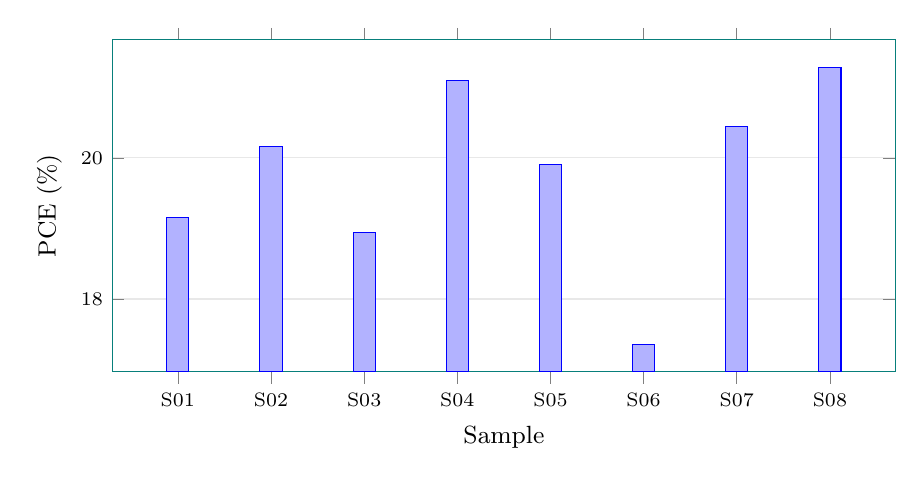
\begin{tikzpicture}\begin{axis}[width=0.95\linewidth,height=58mm,ymajorgrids=true,grid style={gray!18},xlabel={Sample},ylabel={PCE (\%)},xtick={1,...,8},xticklabels={S01,S02,S03,S04,S05,S06,S07,S08},tick label style={font=\scriptsize},label style={font=\small},bar width=8pt,ybar,fill=LabAccent,draw=LabAccent]\addplot coordinates {(1,19.15) (2,20.16) (3,18.94) (4,21.1) (5,19.9) (6,17.36) (7,20.44) (8,21.28)};\end{axis}\end{tikzpicture}\end{center}
\scriptsize\begin{longtable}{@{}lllrrrrrr@{}}\toprule Sample & Formulation & Batch & Voc & Jsc & FF & PCE & Stability & Hyst. \\ \midrule\endhead
S01 & FA0.85MA0.15 & B01 & 1.08 & 22.7 & 78.1 & 19.15 & 89 & 3.2 \\
S02 & FA0.85MA0.15 & B01 & 1.10 & 23.2 & 79.0 & 20.16 & 91 & 2.8 \\
S03 & FA0.80MA0.20 & B02 & 1.07 & 22.9 & 77.3 & 18.94 & 85 & 4.1 \\
S04 & FA0.90MA0.10 & B03 & 1.12 & 23.5 & 80.2 & 21.10 & 94 & 2.1 \\
S05 & FA0.90MA0.10 & B03 & 1.09 & 23.0 & 79.4 & 19.90 & 92 & 2.5 \\
S06 & FA0.75MA0.25 & B04 & 1.05 & 21.8 & 75.8 & 17.36 & 78 & 5.9 \\
S07 & FA0.85MA0.15 & B05 & 1.11 & 23.1 & 79.7 & 20.44 & 90 & 2.7 \\
S08 & FA0.90MA0.10 & B06 & 1.13 & 23.4 & 80.5 & 21.28 & 95 & 1.9 \\
\bottomrule\end{longtable}\normalsize

\section{Evidence-Linked Findings}

\begin{itemize}
\item \textbf{FA0.90MA0.10 is the strongest candidate} — S04 and S08 lead both PCE and stability, with the lowest hysteresis. \textit{Evidence: S04, S08 · 7 metrics; status: accepted}
\item \textbf{S06 is a multi-metric outlier} — PCE, fill factor and stability are jointly below the robust cohort range; review fabrication notes before exclusion. \textit{Evidence: S06 · IQR + robust z; status: review}
\item \textbf{Batch effect is smaller than formulation effect} — Within-batch variation is limited compared with the shift between formulations. \textit{Evidence: Grouped comparison; status: accepted}
\item \textbf{Stability and hysteresis are inversely associated} — Lower hysteresis appears in the most stable devices; the sample count does not support a causal claim. \textit{Evidence: Spearman preview; status: review}
\item \textbf{Two metadata gaps limit reproducibility} — Humidity during coating and elapsed time before annealing are missing for B04 and B05. \textit{Evidence: Process records; status: action}
\end{itemize}
\textit{AI-assisted findings are advisory and remain separate from researcher-authored conclusions.}

\section{Discussion, Conclusions and Limitations}

\subsection{Discussion}
The current cohort supports validation but not causal inference.
\subsection{Conclusions}
S04 and S08 proceed to validation; S06 remains under review.
\subsection{Limitations}
Small demonstration cohort; no causal inference.

\section{Additional notes}

The author requested one additional validation run.

\section{Provenance and Approval}

\begin{tabularx}{\linewidth}{@{}>{\bfseries}lX@{}}\toprule Data class & Source and control \\ \midrule Raw measurements & Source files remain immutable and linked to sample identifiers.\\ Processed results & Deterministic transformations and grouped statistics.\\ Model/AI output & Model, dataset, prompt, tools and review state remain explicit.\\ Report state & Generated from the current Composer draft.\\ Approval & Pending researcher signature\\ \bottomrule\end{tabularx}
\vspace{6mm}
\textbf{Sources:} batch\_B03\_forward.csv; process\_metadata.yaml; SOL-B04; STK-003/v2.

\end{document}
